% Options for packages loaded elsewhere
\PassOptionsToPackage{unicode}{hyperref}
\PassOptionsToPackage{hyphens}{url}
\documentclass[
  ignorenonframetext,
]{beamer}
\newif\ifbibliography
\usepackage{pgfpages}
\setbeamertemplate{caption}[numbered]
\setbeamertemplate{caption label separator}{: }
\setbeamercolor{caption name}{fg=normal text.fg}
\beamertemplatenavigationsymbolsempty
% remove section numbering
\setbeamertemplate{part page}{
  \centering
  \begin{beamercolorbox}[sep=16pt,center]{part title}
    \usebeamerfont{part title}\insertpart\par
  \end{beamercolorbox}
}
\setbeamertemplate{section page}{
  \centering
  \begin{beamercolorbox}[sep=12pt,center]{section title}
    \usebeamerfont{section title}\insertsection\par
  \end{beamercolorbox}
}
\setbeamertemplate{subsection page}{
  \centering
  \begin{beamercolorbox}[sep=8pt,center]{subsection title}
    \usebeamerfont{subsection title}\insertsubsection\par
  \end{beamercolorbox}
}
% Prevent slide breaks in the middle of a paragraph
\widowpenalties 1 10000
\raggedbottom
\AtBeginPart{
  \frame{\partpage}
}
\AtBeginSection{
  \ifbibliography
  \else
    \frame{\sectionpage}
  \fi
}
\AtBeginSubsection{
  \frame{\subsectionpage}
}
\usepackage{iftex}
\ifPDFTeX
  \usepackage[T1]{fontenc}
  \usepackage[utf8]{inputenc}
  \usepackage{textcomp} % provide euro and other symbols
\else % if luatex or xetex
  \usepackage{unicode-math} % this also loads fontspec
  \defaultfontfeatures{Scale=MatchLowercase}
  \defaultfontfeatures[\rmfamily]{Ligatures=TeX,Scale=1}
\fi
\usepackage{lmodern}
\ifPDFTeX\else
  % xetex/luatex font selection
\fi
% Use upquote if available, for straight quotes in verbatim environments
\IfFileExists{upquote.sty}{\usepackage{upquote}}{}
\IfFileExists{microtype.sty}{% use microtype if available
  \usepackage[]{microtype}
  \UseMicrotypeSet[protrusion]{basicmath} % disable protrusion for tt fonts
}{}
\makeatletter
\@ifundefined{KOMAClassName}{% if non-KOMA class
  \IfFileExists{parskip.sty}{%
    \usepackage{parskip}
  }{% else
    \setlength{\parindent}{0pt}
    \setlength{\parskip}{6pt plus 2pt minus 1pt}}
}{% if KOMA class
  \KOMAoptions{parskip=half}}
\makeatother
\usepackage{graphicx}
\makeatletter
\newsavebox\pandoc@box
\newcommand*\pandocbounded[1]{% scales image to fit in text height/width
  \sbox\pandoc@box{#1}%
  \Gscale@div\@tempa{\textheight}{\dimexpr\ht\pandoc@box+\dp\pandoc@box\relax}%
  \Gscale@div\@tempb{\linewidth}{\wd\pandoc@box}%
  \ifdim\@tempb\p@<\@tempa\p@\let\@tempa\@tempb\fi% select the smaller of both
  \ifdim\@tempa\p@<\p@\scalebox{\@tempa}{\usebox\pandoc@box}%
  \else\usebox{\pandoc@box}%
  \fi%
}
% Set default figure placement to htbp
\def\fps@figure{htbp}
\makeatother
\setlength{\emergencystretch}{3em} % prevent overfull lines
\providecommand{\tightlist}{%
  \setlength{\itemsep}{0pt}\setlength{\parskip}{0pt}}
\usepackage{bookmark}
\IfFileExists{xurl.sty}{\usepackage{xurl}}{} % add URL line breaks if available
\urlstyle{same}
\hypersetup{
  pdftitle={Topos-Theoretic Bridges},
  hidelinks,
  pdfcreator={LaTeX via pandoc}}

\title{\texorpdfstring{Topos-Theoretic
Bridges}{Topos-Theoretic Bridges}}
\author{\texorpdfstring{}{}}
\date{}

\begin{document}
\frame{\titlepage}

\section{Topos-Theoretic Bridges and Inter-Theoretic
Transfer}\label{sec:topos-theory}

\begin{frame}{From Categories to Toposes: The Translation Problem}
\protect\phantomsection\label{from-categories-to-toposes-the-translation-problem}
The preceding sections have shown how case systems, categorial grammars,
distributional semantics, and enriched categories each provide a
different ``window'' onto the same underlying linguistic phenomenon. But
how do we know that results proved in one framework transfer to another?
This is the problem of \emph{inter-theoretic translation}---and it is
precisely the problem that Caramello's {[}-@caramello2016bridges{]}
topos-theoretic bridge technique was designed to solve.
\end{frame}

\begin{frame}{Classifying Toposes and Morita Equivalence}
\protect\phantomsection\label{classifying-toposes-and-morita-equivalence}
\begin{block}{What Is a Topos? Generalized Universes of Sets}
\protect\phantomsection\label{what-is-a-topos-generalized-universes-of-sets}
A \textbf{topos} is a category that behaves like a generalized universe
of sets: it has products, exponentials, a subobject classifier (playing
the role of a ``truth-value object''), and enough structure to interpret
first-order logic internally. The category \textbf{Set} of ordinary sets
is a topos, but there are many others---presheaf categories, sheaf
categories over topological spaces, and the categories of models of
geometric theories.
\end{block}

\begin{block}{Classifying Toposes of Geometric Theories}
\protect\phantomsection\label{classifying-toposes-of-geometric-theories}
Every \emph{geometric theory} \(\mathbb{T}\) (a theory axiomatized by
sequents involving only finite conjunctions, arbitrary disjunctions, and
existential quantification) has a \textbf{classifying topos}
\(\mathcal{E}_\mathbb{T}\)---a canonical topos whose models correspond
exactly to the geometric functors from \(\mathcal{E}_\mathbb{T}\) to
other toposes. The classifying topos encodes the theory's ``logical
shape'' independently of any particular model.

Caramello's key insight {[}-@caramello2016bridges;
-@caramello2021five{]} is that different theories can share the same
classifying topos up to equivalence---an equivalence known as
\textbf{Morita equivalence}. When two theories \(\mathbb{T}_1\) and
\(\mathbb{T}_2\) are Morita equivalent
(\(\mathcal{E}_{\mathbb{T}_1} \simeq \mathcal{E}_{\mathbb{T}_2}\)), any
property that can be expressed as an invariant of the classifying topos
transfers automatically between them.
\end{block}
\end{frame}

\begin{frame}{Bridge Theorems for the Four Case Theories}
\protect\phantomsection\label{bridge-theorems-for-the-four-case-theories}
\begin{block}{Formalizing Case Theories as Geometric Theories}
\protect\phantomsection\label{formalizing-case-theories-as-geometric-theories}
We formalize each case-theoretic framework as a geometric theory:

\begin{enumerate}
\item
  \textbf{Typological case theory} \(\mathbb{T}_{\text{typ}}\): Objects
  are case roles, morphisms are grammatical relations, axioms specify
  alignment constraints (e.g., ``S = A'' in accusative alignment).
\item
  \textbf{Type-logical case theory} \(\mathbb{T}_{\text{log}}\): Objects
  are syntactic types, morphisms are Lambek calculus derivations, axioms
  specify well-formedness conditions (pregroup contractions).
\item
  \textbf{Distributional case theory} \(\mathbb{T}_{\text{dist}}\):
  Objects are vector spaces, morphisms are linear maps, axioms specify
  the composition law for distributional meaning (DisCoCat).
\item
  \textbf{Enriched case theory} \(\mathbb{T}_{\text{enr}}\): Objects are
  expressions, morphisms carry \([0,1]\)-valued weights, axioms specify
  the identity and composition inequalities.
\end{enumerate}
\end{block}

\begin{block}{The Bridge Theorem: Morita Equivalence Chain}
\protect\phantomsection\label{the-bridge-theorem-morita-equivalence-chain}
The central claim is that these four theories are related by a chain of
Morita equivalences:

\[\mathcal{E}_{\mathbb{T}_{\text{typ}}} \leftarrow \mathcal{E}_{\mathbb{T}_{\text{bridge}}} \rightarrow \mathcal{E}_{\mathbb{T}_{\text{log}}} \leftarrow \mathcal{E}_{\mathbb{T}_{\text{bridge}'}} \rightarrow \mathcal{E}_{\mathbb{T}_{\text{dist}}}\]

where the intermediate toposes are constructed by finding geometric
theories that are simultaneously interpretable in both flanking
frameworks. The Morita equivalence ensures that:

\begin{itemize}
\tightlist
\item
  \textbf{Syntactic theorems port to semantics}: A commutativity result
  proved in the type-logical framework automatically yields a
  compositionality result in the distributional framework.
\item
  \textbf{Typological universals constrain distributional models}:
  Alignment types (accusative, ergative) impose structural constraints
  on the vector spaces used in DisCoCat.
\item
  \textbf{Enriched structure enriches all frameworks}: The
  \([0,1]\)-valued weights from the enriched theory can be pulled back
  to give probabilistic interpretations of typological, logical, and
  distributional constructions.
\end{itemize}

\autoref{fig:functor-alignment} visualizes the alignment functor between
the Accusative and Ergative category instantiations, showing how the
same eight case roles are connected by different morphism structures
under different alignment types.

\begin{figure}
\centering
\pandocbounded{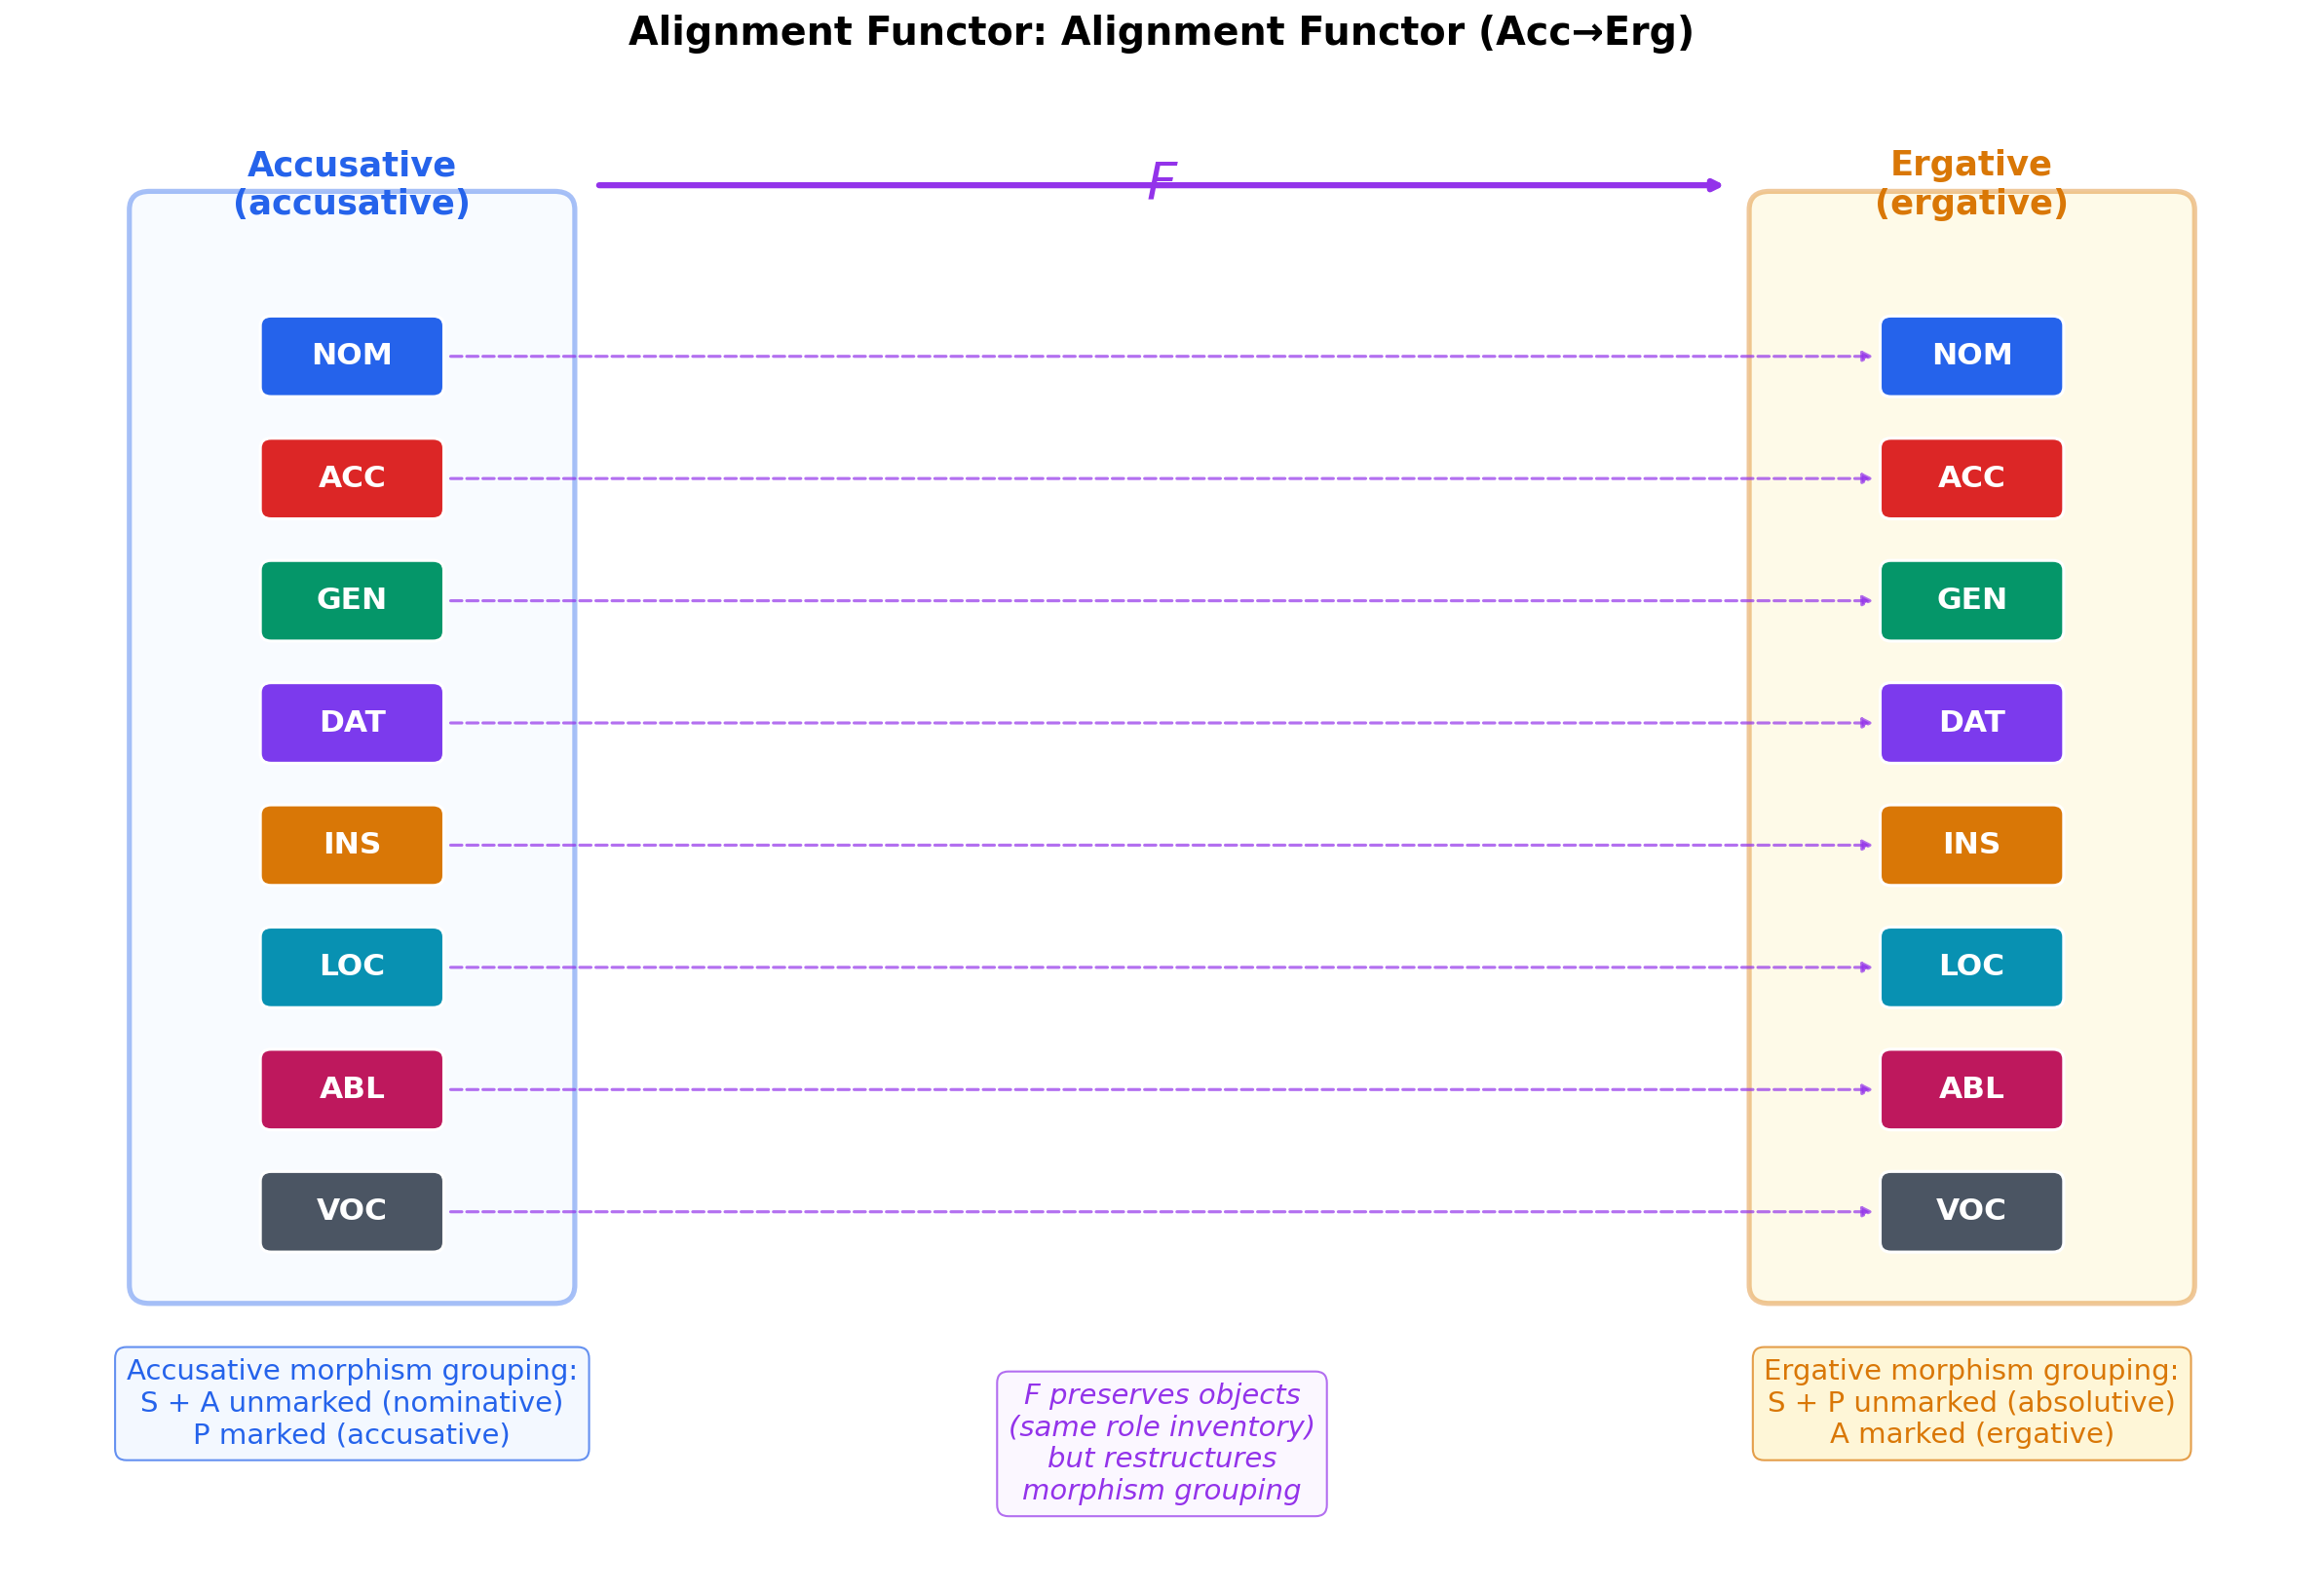
\includegraphics[keepaspectratio,alt={The alignment functor F mapping the Accusative case category (source, blue panel) to the Ergative case category (target, amber panel). Each of the eight case roles (NOM, ACC, GEN, DAT, INS, LOC, ABL, VOC) appears as a labeled node in both categories, with purple horizontal arrows showing the functor's object-level mapping F(role). Below each category, annotations indicate the distinctive morphism grouping: Accusative groups S+A vs.~P (subject and agent unmarked); Ergative groups S+P vs.~A (absolutive unmarked). An explanatory legend clarifies that the functor preserves role inventory but restructures the morphism pattern --- the formal content of the alignment-as-functor principle.}]{../figures/functor_alignment.png}}
\caption{The alignment functor F mapping the Accusative case category
(source, blue panel) to the Ergative case category (target, amber
panel). Each of the eight case roles (NOM, ACC, GEN, DAT, INS, LOC, ABL,
VOC) appears as a labeled node in both categories, with purple
horizontal arrows showing the functor's object-level mapping F(role).
Below each category, annotations indicate the distinctive morphism
grouping: Accusative groups S+A vs.~P (subject and agent unmarked);
Ergative groups S+P vs.~A (absolutive unmarked). An explanatory legend
clarifies that the functor preserves role inventory but restructures the
morphism pattern --- the formal content of the alignment-as-functor
principle.}\label{fig:functor-alignment}
\end{figure}
\end{block}
\end{frame}

\begin{frame}{Phillips and the Universal Language of Thought}
\protect\phantomsection\label{phillips-and-the-universal-language-of-thought}
Phillips {[}-@phillips2024lot{]} provides a striking application of
topos-theoretic methods to cognitive science. He shows that the
\textbf{Language of Thought} (LoT) hypothesis---the claim that cognition
operates over structured, combinatorial representations with
language-like properties---can be formalized categorically, and that the
resulting structure is \emph{universal} in the topos-theoretic sense.

Specifically, Phillips demonstrates that:

\begin{enumerate}
\item
  LoT properties (discrete constituents, role-filler independence,
  systematicity) arise as \textbf{universal constructions} in a
  topos---categorical products, fiber bundles, and presheaves.
\item
  Every topos supports an internal first-order logic, explaining how
  LoT-like logical capacities can emerge in systems (biological or
  artificial) whose internal architecture forms a topos.
\item
  The ``shape'' of cognitive representations is fundamentally
  \textbf{topological}, captured by presheaves and fiber bundles rather
  than by point-set structures.
\end{enumerate}

For our framework, Phillips's result is significant because it provides
a topos-theoretic foundation for the claim that case structure is a
universal feature of cognitive architecture. If the Language of Thought
is topos-universal, and case categories are definable within any topos
(which they are, being small categories with first-order axioms), then
every cognitive system with LoT-like structure must be able to represent
case distinctions---a strong universality claim that goes beyond mere
typological observation.
\end{frame}

\begin{frame}{Syntactic Learning via Classifying Toposes}
\protect\phantomsection\label{syntactic-learning-via-classifying-toposes}
Caramello {[}-@caramello2023syntactic{]} extends the bridge technique to
a learning theory: she shows that classifying toposes can be used to
\emph{learn} the theory of a mathematical structure from finite data (a
finite set of models). The learning algorithm constructs a classifying
topos from the observed data and then extracts the axioms of the
underlying theory.

Applied to case systems, this suggests a principled approach to
\emph{grammatical induction}: given a corpus annotated with case labels,
one could construct the classifying topos of the implicit case theory
and read off its axioms---recovering the alignment type, the morphism
structure, and the enriched weights from data alone. This
topos-theoretic learning procedure would be provably correct (recovering
the true theory in the limit) and maximally general (not presupposing
any particular alignment type).
\end{frame}

\begin{frame}{Diagrammatic Implications of Inter-Theoretic Transfer}
\protect\phantomsection\label{diagrammatic-implications-of-inter-theoretic-transfer}
The bridge technique has a natural diagrammatic interpretation. Morita
equivalence between theories is witnessed by \emph{functorial
translations}---diagrams in the 2-category of toposes that commute up to
natural isomorphism. These diagrams serve the same cognitive function as
the commutative diagrams of \autoref{sec:introduction}: they make the
transfer of structure visible, allowing a researcher to verify at a
glance that a result proved in one framework genuinely applies in
another.

Manders {[}-@manders2008euclidean{]} observed that even in classical
mathematics, diagrams serve not merely as illustrations but as
\emph{inferential instruments} whose spatial properties encode
proof-relevant information. The topos-theoretic bridge diagrams extend
this observation to the meta-theoretical level: the commutative diagram
expressing Morita equivalence is itself a ``free ride'' inference,
automatically transferring any topos-invariant property from one theory
to another without requiring a case-by-case verification.
\end{frame}

\end{document}
